%%%%%%%%%%%%%%%%%%%%%%%%%%%%%%%%%%%%%%%%%%%%%%%%%%%%%%%%%%%%%%%%%%%%%
%
% Complete documentation on the extended LaTeX markup used for Insight
% documentation is available in ``Documenting Insight'', that is part
% of the standard documentation for Insight.  It may be found online
% at:
%
%                    http://www.itk.org
%
%%%%%%%%%%%%%%%%%%%%%%%%%%%%%%%%%%%%%%%%%%%%%%%%%%%%%%%%%%%%%%%%%%%%%

\documentclass{InsightSoftwareGuide}

\usepackage[pdftex]{graphicx}

\usepackage{times,lscape,url}

\usepackage[latin1]{inputenc}

\usepackage{tikz}

\usepackage{color}

\usepackage{xspace}

\usepackage{longtable}

\definecolor{listcomment}{rgb}{0.0,0.5,0.0}
\definecolor{listkeyword}{rgb}{0.0,0.0,0.5}
\definecolor{listnumbers}{gray}{0.65}
\definecolor{listlightgray}{gray}{0.955}
\definecolor{listwhite}{gray}{1.0}

\usepackage{listings}

\newcommand{\lstsetcpp}
{
\lstset{frame = tb,
       framerule = 0.25pt,
       float,
       fontadjust,
       backgroundcolor={\color{listlightgray}},
       basicstyle = {\ttfamily\footnotesize},
       keywordstyle = {\ttfamily\color{listkeyword}\textbf},
       identifierstyle = {\ttfamily},
       commentstyle = {\ttfamily\color{listcomment}\textit},
       stringstyle = {\ttfamily},
       showstringspaces = false,
       showtabs = false,
       numbers = none,
       numbersep = 6pt,
       numberstyle={\ttfamily\color{listnumbers}},
       tabsize = 2,
       language=[ANSI]C++,
       floatplacement=!h
       }
}
\newcommand{\lstsetpython}
{
\lstset{language=Python
        }
}
\newcommand{\lstsetjava}
{
\lstset{language=Java
        }
}


\newif\ifitkFullVersion
\itkFullVersiontrue
%\itkFullVersionfalse

\newif\ifitkPrintedVersion
\itkPrintedVersiontrue
%\itkPrintedVersionfalse

%%%%%%%%%%%%%%%%%%%%%%%%%%%%%%%%%%%%%%%%%%%%%%%%%%%%%%%%%%%%%%%%%%
%
%  hyperref should be the last package to be loaded.
%
%%%%%%%%%%%%%%%%%%%%%%%%%%%%%%%%%%%%%%%%%%%%%%%%%%%%%%%%%%%%%%%%%%
\usepackage[
pdftitle={The Orfeo ToolBox Cookbook, a guide for non-developers},
pdfauthor={CNES},
pdfsubject={Remote Sensing, Orfeo, Pleiades, Cosmo Skymed},
pdfkeywords={image processing, Remote sensing, Guide},
pdfpagemode={UseOutlines},
bookmarks,bookmarksopen,
pdfstartview={FitH},
backref,
colorlinks,linkcolor={red},citecolor={blue},urlcolor={blue},
]{hyperref}

\usepackage{amsmath,amssymb,amsfonts}
\usepackage{bbm}



\def\logoCNES{../Art/CNES_nom.pdf}



% Useful macros
\newcommand{\otb}{\textbf{Orfeo ToolBox}\xspace}
\newcommand{\app}{\textbf{OTB Applications}\xspace}
\newcommand{\mont}{\textbf{Monteverdi}\xspace}
\newcommand{\jpg}{\href{http://en.wikipedia.org/wiki/JPEG_2000}{Jpeg2000}\xspace}
\newcommand{\phr}{\href{http://smsc.cnes.fr/PLEIADES/index.htm}{Pleiades}\xspace}
\newcommand{\mmod}[1]{\emph{#1}\index{#1}\xspace}
\newcommand{\application}[1]{\emph{#1}\index{#1}\xspace}
\newcommand{\ossim}{\href{http://www.ossim.org/OSSIM/OSSIM_Home.html}{OSSIM}\xspace}
\newcommand{\sg}{\href{http://orfeo-toolbox.org/SoftwareGuide/}{OTB Software Guide}\xspace}
\newcommand{\dox}{\href{http://orfeo-toolbox.org/doxygen/}{Doxygen}\xspace}
\newcommand{\website}{\href{http://orfeo-toolbox.org}{Orfeo ToolBox website}\xspace}
\newcommand{\qgis}{\href{http://www.qgis.org/}{Quantum GIS}\xspace}
\newcommand{\gdal}{\href{http://www.gdal.org/}{GDAL}\xspace}
\newcommand{\osgeow}{\href{http://trac.osgeo.org/osgeo4w/}{OSGeo4W}\xspace}
\newcommand{\download}{\href{https://www.orfeo-toolbox.org/download/}{OTB download
   page}\xspace}
\newcommand{\googleearth}{\textbf{Google Earth\copyright}\xspace}

\newtheorem{algo}{Algorithm}
\newtheorem{defin}{Definition}

\title{The Orfeo ToolBox Cookbook, a guide for non-developers\\ Updated
  for OTB-5.4.0}

\author{OTB Development Team}

\authoraddress{
  \url{http://www.orfeo-toolbox.org}\\
  e-mail: \email{otb@cnes.fr}
}

\date{\today}


% actually write the .idx file
\makeindex

\setcounter{tocdepth}{3}

%%%%%%%%%%%%%%%%%%%%%%%%%%%%%%%%%%%%%%%%%%%%%%%%%%%%%%%%%%%%%%%%%%%
%
%           Begin Document
%
%%%%%%%%%%%%%%%%%%%%%%%%%%%%%%%%%%%%%%%%%%%%%%%%%%%%%%%%%%%%%%%%%%%

\begin{document}

\ifitkPrintedVersion
\fi

\maketitle

\frontmatter

\hyperbaseurl{http://www.orfeo-toolbox.org}

\lstsetcpp

%%%%%%%%%%%%%%%%%%%%%%%%%%%%%%%%%%%%%%%%%%
%
%  Page with OTB logo
%
%%%%%%%%%%%%%%%%%%%%%%%%%%%%%%%%%%%%%%%%%%
\cleardoublepage

\begin{minipage}[t][10cm][b]{\textwidth}
\center
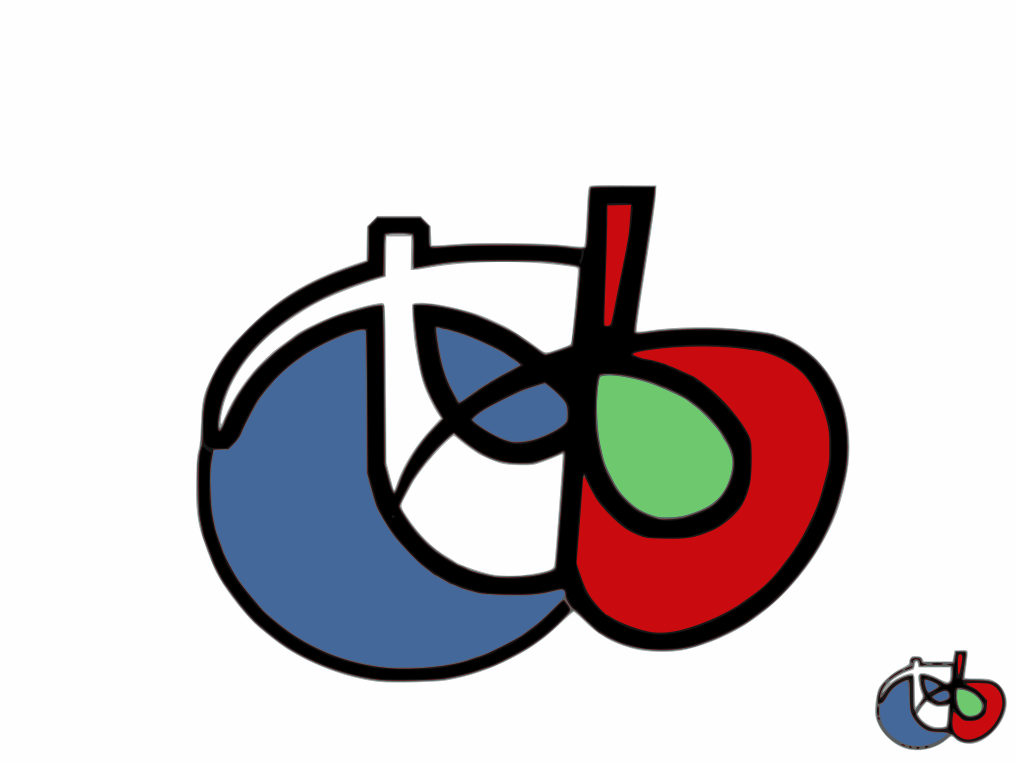
\includegraphics[width=0.5\textwidth]{../Art/logoVectoriel.pdf}
\large
\begin{center}
\emph{The ORFEO Toolbox is not a black box.}\\
\end{center}
\hspace{8cm} Ch.D.
\normalsize
\end{minipage}

%%%%%%%%%%%%%%%%%%%%%%%%%%%%%%%%%%%%%%%%%%%%%%
%
% remove headings from the following material
\pagestyle{plain}
%
%%%%%%%%%%%%%%%%%%%%%%%%%%%%%%%%%%%%%%%%%%%%%%

%%\ifitkPrintedVersion
%% \input{Cover.tex}
%%\fi

%\input{Abstract.tex}
\chapter*{Foreword}
\noindent
After almost 5 years of development, the \otb has become a
rich library used in many remote sensing context, from research work
to operational systems. The \app and more recently the
Monteverdi tool has helped to broaden the audience of the library,
giving access to its functionalities to non-developers.

Meanwhile, the \sg has grown to more
than 700 pages of documented code examples, which, combined with the
class documentation with the \dox, allows developer users to find
their way through the \otb so as to write code suiting their
needs.

Yet, the documentation available for non-developers users, using
Monteverdi and \app to perform everyday remote sensing tasks, has been
almost inexistent for all these years, and these users had to learn
the software by themselves or ask for help from more experienced
users. This cookbook aims at fulfilling the need for an appropriate
documentation of the applications built upon the \otb: \mont, and
\app, which are now integrated into the main \otb package and provide
several access mode (command-line, QT interface, QGis plugins, other
languages \ldots).

A general introduction to these tools is first presented, along
with installation instructions. Rather than describing all modules and
applications in an exhaustive way, we then decided to focus on very
common remote sensing tasks, detailing how they can be achieved with
either \mont or an application.

For more information on the \otb, please feel free to visit the \website.

%%%%%%%%%%%%%%%%%%%%%%%%%%%%%%%%%%%%%%%%%%%%%%%%%%%%%%%%%
%
% Insert Table of Contents; List of Figures and Tables
%
%%%%%%%%%%%%%%%%%%%%%%%%%%%%%%%%%%%%%%%%%%%%%%%%%%%%%%%%%


%%%%%%%%%%%%%%%%%%%%%%%%%%%%%%%%%%%%%%%%%%%%%%
%
% enable headings from the following material
\pagestyle{normal}
%
%%%%%%%%%%%%%%%%%%%%%%%%%%%%%%%%%%%%%%%%%%%%%%
\small
\tableofcontents
\listoffigures
\listoftables
\normalsize

%%%%%%%%%%%%%%%%%%%%%%%%%%%%%%%%%%%%%%%%%
%
% Begin technical content
%
%%%%%%%%%%%%%%%%%%%%%%%%%%%%%%%%%%%%%%%%%

\mainmatter

\chapter{A brief tour of OTB-Applications}\label{chap:otb-applications}

\section{Introduction}\label{sec:appintro}

\app was perhaps the older package of the \otb suite after the OTB
package itself. Since the \otb is a library providing remote sensing
functionalities, the only applications that were distributed at the
beginning were the examples from the Software Guide and the
tests. These applications are very useful for the developer because
their code is very short and only demonstrates one functionality at a
time. In many cases, a real application would require :
\begin{itemize}
\item combining together two or more functions from the \otb
\item providing a nice high level interface to handle : parameters, input data,
output data and communication with the user
\end{itemize}

The \app package was originally designed to provide applications
performing simple remote sensing tasks, more complex than simple
examples from the Software Guide, and with a more user-friendly
interface (either graphical or command-line), to demonstrate the use
of the \otb functions. The most popular applications are maybe the
\application{otbImageViewerManager}, which allows to open a collection
of images and navigate in them, and the
\application{otbSupervisedClassificationApplication}, which allowed to
delineate training regions of interest on the image and classify the
image with a SVM classifier trained with these regions (this
application is no longer maintained since the same functionnality is
available through the corresponding \mont module). During the first 3
years of the \otb development, many more applications have been added
to this package, to perform various tasks. Most of them came with a
graphical user interface, apart from some small utilities that are
command-line.

The development and release of the \mont software (see
chapter~\ref{chap:Monteverdi} at the end of year 2009 changed a lot of
things for the \app package: most of non-developer users were looking
for quite a long time for an application providing \otb
functionalities under a unified graphical interface. Many applications
from the \app package were integrated to \mont as modules, and the
\app package lost a lot of its usefulness. No more applications were
added to the package and it was barely maintained, as new graphical
tools were directly embedded within \mont.

Then, some people started to regain interest in the \app
package. \mont is a great tool to perform numerous remote sensing and
image processing task in a minute, but it is not well adapted to
heavier (and longer) processing, scripting and batch
processing. Therefore, in 2010 the \app package has been revamped: old
applications have been moved to a legacy folder for backward
compatibility, and the development team started to populate the
package with compact command-line tools to perform various heavy
processing tasks. 

Later on in 2011, the \app has been further revamped. Because of the
increasing need to interface the \app into other software and to
provide auto-generated interfaces, the \otb development team decided
to develop a new application framework. The main idea of this
framework is the following: each application is written once for all
in a shared library (also known as plugin). This plugin can be
auto-loaded into appropriate tools wihtout recompiling, and is able to
fully describe its parameters, behaviour and documentation.

The tools to use the plugins can be extended, but \otb shipped the
following:
\begin{itemize}
\item A command-line laucher, which is almost equivalent to the former
  \app command-line interface,
\item A graphical launcher, with an auto-generated QT interface,
  providing ergonomic parameters setting, display of documentation,
  and progress reporting,
\item A SWIG interface, which means that any application can be
  loaded set-up and executed into a high-level language such as Python
  or Java for instance.
\end{itemize}

Additionally, \href{http://www.qgis.org/}{QGis} plugins built on top of the SWIG/Python interface
are available with seamless integration within QGis. You can find a short guide about it \href{http://wiki.orfeo-toolbox.org/index.php/Quantum_GIS_access_to_OTB_applications}{here}.

To facilitate the use of these tools and applications, they will now
be shipped with the standard \otb package. It means that the former
\textbf{OTB-Applications} package has entered its maintenance cycle :
no new feature will be pushed there, and all development is done directly
inside the \otb paackage.

The \app are now rich of more than 40 tools, which are listed in the
the applications reference documentation, presented in
chapter~\ref{chap:apprefdoc}, page~\pageref{chap:apprefdoc}.

\section{Installation}\label{sec:appinstall}

Since \app are now included within the standard \otb package, their 
installation is made while installing the whole \otb. Detailed 
instructions on how to install the whole \otb suite either from 
binary packages or from source are available in the \sg. 

Here, we will focus only on the installation of the new \app package.

\subsection{Windows 2000/XP/Vista/Seven}
\label{ssec:app_windows_binaries}

For Windows 2000/XP/Vista/Seven users, we recommend to use the package \textbf{otb-bin} available through \osgeow which will manage the dependencies. This package provides all the applications through the command-line launcher and the Qt interface. They will be available directly in the OSGeo4W shell. For example after finishing the installation you can run in the OSGeo4W shell:
\begin{verbatim}
otbgui_Smoothing
\end{verbatim}
to check the installation of the new \app.

\subsection{MacOS X}
\label{ssec:mac_binaries}

For now, no binary package is available for \app on MacOS X. You can build the \app from sources by following instructions in the \sg with the option \code{BUILD\_APPLICATIONS=ON}.

\subsection{Linux}

\subsubsection{Ubuntu 10.04, 10.10, 11.10 and 12.04}
\label{ssec:ubuntu_binaries}
For Unbuntu 10.04 (Lucid Lynx), 10.10 (Maverick Meerkat), 11.10 (Oneiric Ocelot) and 12.04 (Precise Pangolin) , the whole \otb suite and  specifically the \app are available through APT repositories. The generation of packages for 11.04 (Natty Narwhal) are suspended because some packages are not yet available. 

If you are using apt command-line tools, use these command-lines to add the otb repository to apt sources:
\begin{verbatim}
sudo aptitude install add-apt-repository 
sudo add-apt-repository ppa:otb/orfeotoolbox-stable
\end{verbatim}
Now run:
\begin{verbatim}
sudo aptitude update
sudo aptitude install otb-bin otb-bin-qt otb-python
\end{verbatim}

If you are using \emph{Synaptic}, you can add the repositories, update and install the packages through the graphical interface.

If you want to use OTB with bleeding edge versions of gdal and qgis,
there is an alternate UbuntuGIS repository.  You can add it by using
these command-lines:
\begin{verbatim}
sudo aptitude install add-apt-repository 
sudo apt-add-repository ppa:ubuntugis/ubuntugis-unstable
sudo add-apt-repository ppa:otb/orfeotoolbox-stable-ubuntugis
\end{verbatim}
Now run:
\begin{verbatim}
sudo aptitude update
sudo aptitude install otb-bin otb-bin-qt otb-python
\end{verbatim}

Be careful not to add the two repositories, since they may cause incompatibilities.

For further informations about ubuntu packages go to
\href{https://launchpad.net/~otb/+archive/orfeotoolbox-stable}{orfeotoolbox-stable
  launchpad page} and click on \textbf{Read about installing}.

\textbf{apt-add-repository} will try to retrieve the GPG keys of the
repositories to certify the origin of the packages. If you are behind
a http proxy, this step won't work and apt-add-repository will stall
and eventually quit. You can temporarily ignore this error and proceed
with the update step. Following this, aptitude update will issue a
warning about a signature problem. This warning won't prevent you from
installing the packages.

\subsubsection{OpenSuse 11.2 and higher}
\label{ssec:opensuse_binaries}

For OpenSuse 11.2 and higher, the whole \otb suite is available
through \emph{zypper}.

First, you need to add the appropriate repositories with these
command-lines (please replace $11.4$ by your OpenSuse version):
\begin{verbatim}
sudo zypper ar 
http://download.opensuse.org/repositories/games/openSUSE_11.4/ Games
sudo zypper ar 
http://download.opensuse.org/repositories/Application:/Geo/openSUSE_11.4/ GEO
sudo zypper ar 
http://download.opensuse.org/repositories/home:/tzotsos/openSUSE_11.4/ tzotsos
\end{verbatim}

Now run:
\begin{verbatim}
sudo zypper refresh
sudo zypper install Orfeo-Applications
\end{verbatim}

Alternatively you can use the One-Click Installer from the
\href{http://software.opensuse.org/search?q=Orfeo&baseproject=openSUSE\%3A11.4&lang=en&include_home=true&exclude_debug=true}{openSUSE
  Download page} or add the above repositories and install through
Yast Package Management.

In case you wish to test the latest version of the packages, you can run:
\begin{verbatim}
sudo zypper refresh
sudo zypper install Orfeo-Applications-beta
\end{verbatim}


\section{Using the applications}\label{sec:usingapps}

Using the new \app framework is slightly more complex than launching a
command-line tool. This section describes all the ways to launch the
new applications. Apart from the simplified access, which is similar
to the former access to \app, you will need to know the application 
name and optionally the path where the applications plugins are stored.
For applications shipped with \otb, the name of each 
application can be found in chapter~\ref{chap:apprefdoc}, 
page~\pageref{chap:apprefdoc}.

\subsection{Simplified use}

All standard applications delivered in with \otb comes with simplified
scripts in the system path, allowing to launch the command-line and
 graphical user interface versions of the application in the same simple way
 we used to launch the old applications. The command-line interface is prefixed by
\verb?otbcli_?, while the Qt interface is prefixed by
\verb?otbgui_?. For instance, calling \verb?otbcli_Convert? will
launch the command-line interface of the \textbf{Convert} application,
while \verb?otbgui_Convert? will launch its GUI.

%For Windows users, the simplified Qt interface launcher is also
%available from the Start Menu.

Passing arguments to the command-line version (prefixed by
\verb?otbcli_?) is explained in next sub-section.

\subsection{Using the command-line launcher}

The command-line application launcher allows to load an application
plugin, to set its parameters, and execute it using the command
line. Launching the \verb?otbApplicationLauncherCommandLine?
without argument results in the following help to be displayed:

\begin{verbatim}
$ otbApplicationLauncherCommandLine 
Usage : ./otbApplicationLauncherCommandLine module_name [MODULEPATH] [arguments]
\end{verbatim} 

The \verb?module_name? parameter corresponds to the application
name. The \verb?[MODULEPATH]? argument is optional and allows 
to pass to the launcher a path where the shared library (or plugin) 
corresponding to \verb?module_name? is.

It is also possible to set this path with the environment variable 
\verb?ITK_AUTOLOAD_PATH?, making the \verb?[MODULEPATH]? optional.
This variable is checked by default when 
no \verb?[MODULEPATH]? argument is given.
When using multiple paths in \verb?ITK_AUTOLOAD_PATH?, one must make sure to use
the standard path separator of the target system, which is \verb?:? on Unix, and \verb?;? on Windows.


An error in the application name (i.e. in parameter
\verb?module_name?) will make the
\verb?otbApplicationLauncherCommandLine? lists the name of all
applications found in the available path (either \verb?[MODULEPATH]? 
and/or \verb?ITK_AUTOLOAD_PATH?).

To ease the use of the applications, and try avoiding extensive environment
customization, ready-to-use scripts are provided by the OTB installation
to launch each application, and takes care of adding the standard application
installation path to the \verb?ITK_AUTOLOAD_PATH? environment variable.

These scripts are named \verb?otbcli_<ApplicationName>? and do not need any path
settings. For example you can start the Orthorectification application
with the script called \verb?otbcli_Orthorectification?.


Launching an application with no or incomplete parameters will make the
launcher display a summary of the parameters, indicating the mandatory parameters
missing to allow for application execution. Here is an example
with the \textbf{OrthoRectification} application:

\begin{scriptsize}
\begin{verbatim}
$ otbcli_OrthoRectification

ERROR: Waiting for at least one parameter...

====================== HELP CONTEXT ======================
NAME: OrthoRectification
DESCRIPTION: This application allows to ortho-rectify optical images from supported sensors.

EXAMPLE OF USE: 
otbcli_OrthoRectification -io.in QB_TOULOUSE_MUL_Extract_500_500.tif -io.out QB_Toulouse_ortho.tif

DOCUMENTATION: http://www.orfeo-toolbox.org/Applications/OrthoRectification.html
======================= PARAMETERS =======================
        -progress                        <boolean>        Report progress 
MISSING -io.in                           <string>         Input Image 
MISSING -io.out                          <string> [pixel] Output Image  [pixel=uint8/int8/uint16/int16/uint32/int32/float/double]
        -map                             <string>         Output Map Projection [utm/lambert2/lambert93/transmercator/wgs/epsg]
MISSING -map.utm.zone                    <int32>          Zone number 
        -map.utm.northhem                <boolean>        Northern Hemisphere 
        -map.transmercator.falseeasting  <float>          False easting 
        -map.transmercator.falsenorthing <float>          False northing 
        -map.transmercator.scale         <float>          Scale factor 
        -map.epsg.code                   <int32>          EPSG Code 
        -outputs.mode                    <string>         Parameters estimation modes [auto/autosize/autospacing]
MISSING -outputs.ulx                     <float>          Upper Left X 
MISSING -outputs.uly                     <float>          Upper Left Y 
MISSING -outputs.sizex                   <int32>          Size X 
MISSING -outputs.sizey                   <int32>          Size Y 
MISSING -outputs.spacingx                <float>          Pixel Size X 
MISSING -outputs.spacingy                <float>          Pixel Size Y 
        -outputs.isotropic               <boolean>        Force isotropic spacing by default 
        -elev                            <string>         Elevation management [dem/average]
MISSING -elev.dem.path                   <string>         DEM directory 
        -elev.dem.geoid                  <string>         Geoid File 
        -elev.average.value              <float>          Average Elevation 
        -interpolator                    <string>         Interpolation [nn/linear/bco]
        -interpolator.bco.radius         <int32>          Radius for bicubic interpolation 
        -opt.rpc                         <int32>          RPC modeling (points per axis) 
        -opt.ram                         <int32>          Available memory for processing (in MB) 
        -opt.gridspacing                 <float>          Resampling grid spacing 
\end{verbatim}
\end{scriptsize}


For a detailed description of the application behaviour and
parameters, please check the application reference documentation presented
chapter~\ref{chap:apprefdoc}, page~\pageref{chap:apprefdoc} or
follow the \verb?DOCUMENTATION? hyperlink provided in
\verb?otbApplicationLauncherCommandLine? output. Parameters are passed
to the application using the parameter key (which might include one or
several \verb?.? character), prefixed by a \verb?-?. Command-line
examples are provided in chapter~\ref{chap:apprefdoc},
page~\pageref{chap:apprefdoc}.


\subsection{Using the GUI launcher}

The graphical interface for the applications provides a usefull interactive user interface
to set the parameters, choose files, and monitor the execution progress.

This interface can be activated through the CMake option \code{OTB\_WRAP\_QT}.

This launcher needs the same two arguments as the command line launcher :
\begin{verbatim}
$ otbApplicationLauncherQt module_name [MODULEPATH]
\end{verbatim}

The application paths can be set with the \verb?ITK_AUTOLOAD_PATH? environment variable,
as for the command line launcher.
Also, as for the command-line application, a more simple script is generated and installed by OTB
to ease the configuration of the module path : to launch the \application{Rescale} graphical user interface,
one will start the \verb?otbgui_Rescale? script.

The resulting graphical application displays a window with several tabs:
\begin{itemize}
\item \textbf{Parameters} is where you set the parameters and 
execute the application. 
\item \textbf{Logs} is where you see the informations given by 
the application during its execution. 
\item \textbf{Progress} is where you see a progress bar of the 
execution (not available for all applications). 
\item \textbf{Documentation} is where you find a summary of the 
application documentation.
\end{itemize}

In this interface, every optional parameter has a check box that
you have to tick if you want to set a value and use this parameter.
The mandatory parameters cannot be unchecked.
 
The interface of the application \application{Rescale} is shown 
here as an example.

\begin{figure}[h]
  \center
  \includegraphics[width=0.6\textwidth]{../Art/QtImages/rescale_param.png}
  \itkcaption[GUI of the application Rescale, parameters tab]{Parameters tab in \application{Rescale} application.}
  \label{fig:rescaleParam}
\end{figure}

\begin{figure}[h]
  \center
  \includegraphics[width=0.6\textwidth]{../Art/QtImages/rescale_logs.png}
  \itkcaption[GUI of the application Rescale, logs tab]{Logs tab in \application{Rescale} application.}
  \label{fig:rescaleLogs}
\end{figure}

\begin{figure}[h]
  \center
  \includegraphics[width=0.6\textwidth]{../Art/QtImages/rescale_progress.png}
  \itkcaption[GUI of the application Rescale, progress tab]{Progress tab in \application{Rescale} application.}
  \label{fig:rescaleProgress}
\end{figure}

\begin{figure}[h]
  \center
  \includegraphics[width=0.6\textwidth]{../Art/QtImages/rescale_documentation.png}
  \itkcaption[GUI of the application Rescale, parameters tab]{Parameters tab in \application{Rescale} application.}
  \label{fig:rescaleDocumentation}
\end{figure}

\clearpage

\subsection{Using the Python interface}

The applications can also be accessed from Python, through a module named \verb?otbApplication?

On Unix systems it is typically available in the \verb?/usr/lib/otb/python? directory.
You may need to configure the environment variable \verb?PYTHONPATH? to include this directory
so that the module becomes available from an Python shell.

On Windows, you can install the \verb?otb-python? package, and the module will be available from
an OSGeo4W shell automatically.

In this module, two main classes can be manipulated :
\begin{itemize}
\item \verb?Registry?, which provides access to the list of available applications,
      and can create applications
\item \verb?Application?, the base class for all applications. This allows to interact with an application instance
      created by the \verb?Registry?
\end{itemize}

As for the command line and GUI launchers, the path to the application modules needs to
be properly set with the \verb?ITK_AUTOLOAD_PATH? environment variable.
The standard location on Unix systems is \verb?/usr/lib/otb/applications?.
On Windows, the applications are available in the \verb?otb-bin? OSGeo4W package, and
the environment is configured automatically so you don't need to tweak \verb?ITK_AUTOLOAD_PATH?.

Here is one example of how to use Python to run the \verb?Smoothing? application, changing the algorithm
at each iteration.

\begin{lstlisting}[language=python,breaklines=true,breakatwhitespace=true,frame = tb,framerule = 0.25pt,fontadjust,backgroundcolor={\color{listlightgray}},basicstyle = {\ttfamily\scriptsize},keywordstyle = {\ttfamily\color{listkeyword}\textbf},identifierstyle = {\ttfamily},commentstyle = {\ttfamily\color{listcomment}\textit},stringstyle = {\ttfamily},showstringspaces = false,showtabs = false,numbers = none,numbersep = 6pt, numberstyle={\ttfamily\color{listnumbers}},tabsize = 2]
#  Example on the use of the Smoothing application
#

# We will use sys.argv to retrieve arguments from the command line.
# Here, the script will accept an image file as first argument,
# and the basename of the output files, without extension.
from sys import argv

# The python module providing access to OTB applications is otbApplication
import otbApplication

# otbApplication.Registry can tell you what application are available
print "Available applications : "
print str( otbApplication.Registry.GetAvailableApplications() )

# Let's create the application with codename "Smoothing"
app = otbApplication.Registry.CreateApplication("Smoothing")

# We print the keys of all its parameter
print app.GetParametersKeys()

# First, we set the input image filename
app.SetParameterString("in", argv[1])

# The smoothing algorithm can be set with the "type" parameter key
# and can take 3 values : 'mean', 'gaussian', 'anidif'
for type in ['mean', 'gaussian', 'anidif']:

  print 'Running with ' + type + ' smoothing type'

  # Here we configure the smoothing algorithm
  app.SetParameterString("type", type)

  # Set the output filename, using the algorithm to differenciate the outputs
  app.SetParameterString("out", argv[2] + type + ".tif")

  # This will execute the application and save the output file
  app.ExecuteAndWriteOutput()

\end{lstlisting}






%\chapter{Using OTB applications}\label{chap:WrappedApplications}

\section{Introduction}\label{sec:wrappedAppliIntro}
The \app package (see \ref{chap:otb-applications}) has brought a nice set of 
applications, along with several tools to launch them (command line, Qt,...).
As for the future of these applications, it has been decided to integrate 
them inside the \otb library. This migration has been an opportunity to 
enhance all the framework around the applications: not only new features have
 been added, but the interface with the developer has also been simplified. 
The new framework has inherited the wrappers from \app, and new ones have been
added. The development philosophy behind these applications is to provide users 
with modular functional blocs for remote sensing, ready to be integrated in any
environment. 

Because the applications are now a part of the library, their installation doesn't
require much effort: when building the \otb library, you can activate the applications 
with the CMake boolean option \code{BUILD\_APPLICATIONS}.

\section{List of applications}\label{sec:wrappedAppliList}
The documentation of the available applications is accessible 
\href{http://orfeo-toolbox.org/Applications}{here}. Most of the old applications have
been migrated. They are sorted by categories.

\section{Available wrappers}\label{sec:wrappedAppliWrappers}

\subsection{Command line}\label{sec:wrappedAppliCmdLine}
By default, the applications can be called with the command line launcher. This launcher
is built in your \code{OTB\_DIR/bin} directory. It needs at least two arguments: the 
application name and the path to the \code{OTB\_DIR/bin} directory. Any additional argument
will be given to the application itself. You can ask the application to print its help
message:
\begin{verbatim}
otbApplicationLauncherCommandLine Rescale OTB_DIR/bin -help
\end{verbatim}
The help message (but also the \href{http://orfeo-toolbox.org/Applications}{documentation})
will give you the list of available parameters. Each parameter must be set by giving the 
corresponding key followed by its value:
\begin{verbatim}
otbApplicationLauncherCommandLine Rescale OTB_DIR/bin -in QB_Toulouse_Ortho_PAN.tif -out QB_Toulouse_rescaled.tif -outmin 0 -outmax 255
\end{verbatim}

If the application has sub-parameters (i.e. parameters contained in other parameters), 
their key must be prefixed by their full tree path. For instance, the application 
\code{OrthoRectification} has a paramater for bicubic interpolation radius whose key is \code{radius}.
This parameter should be called with the path \code{-interpolator.bco.radius}.

Note that some types of parameters allow you to give several values after the key (they must
be separated with whitespaces).

\subsection{Other wrappers}\label{sec:wrappedAppliOtherWrap}
If you want to use an other wrapper, you have to activate the corresponding CMake 
options when building the library:
\begin{itemize}
  \item Enable \code{WRAP\_QT} to build a Qt application launcher. It opens a GUI which 
  allows you to set the parameters and execute the application. This launcher only needs 
  the same two arguments as the command line:
  \begin{verbatim}
  otbApplicationLauncherQt Rescale OTB_DIR/bin
  \end{verbatim}
  It displays a window with several tabs. \textbf{[Parameters]} is where you set the parameters and execute the application.
  \textbf{[Logs]} is where you see the informations given by the application during its execution. \textbf{[Progress]} is 
  where you see a progress bar of the execution (not available for all applications). \textbf{[Documentation]} is where you
  find a summary of the application documentation.
   
  \item \code{WRAP\_PYTHON} : \textbf{TODO}
  \item \code{WRAP\_PYQT} : \textbf{TODO}
  \item \code{WRAP\_JAVA} : \textbf{TODO}
\end{itemize}



\chapter{Monteverdi}\label{chap:Monteverdi}

\chapter{Recipes}\label{chap:recipes}

\section{Optical pre-processing}\label{sec:optpreproc}

This section present various pre-processing tasks that can be done
using \app or \mont.

\subsection{Optical radiometric calibration}\label{ssec:optcal}

In remote sensing imagery, pixel values are called DN (for Digital
Numbers) and can not be physically interpreted and compared: they are
influenced by various factors such as the amount of light flowing
trough the sensor, the gain of the detectors and the analogic to
numeric converter.

Depending on the season, the light and atmospheric conditions, to
position of the sun or the sensor internal parameters, these DN can
drastically change for a given pixel (apart from any ground change
effects). Moreover, these effect are not uniform over the spectrum:
for instance aerosol amount and type has usually more impact on the
blue channel.

Therefore, it is necessary to calibrate the pixel values before any
physical interpretation is made out of them. In particular, this
processing is mandatory before any comparison of pixel spectrum
between several images (from the same sensor), and to train a
classifier without dependence to the atmospheric conditions at the
acquisition time.

Calibrated values are called surface reflectivity, which is a ratio
denoting the fraction of light that is reflected by the underlying
surface in the given spectral range. As such, its values lie in the
range $[0,1]$. For convenience, images are often stored in thousandth
of reflectivity, so that they can be encoded with an integer type.
Two levels of calibration are usually distinguished:

\begin{itemize}
\item The first level is called \emph{Top Of Atmosphere (TOA)}
  reflectivity. It takes into account the sensor gain, sensor spectral
  response and the solar illumination.
\item The second level is called \emph{Top Of Canopy (TOC)}
  reflectivity. In addition to sensor gain and solar illumination, it
  takes into account the optical thickness of the atmosphere, the
  atmospheric pressure, the water vapor amount, the ozone amount, as
  well as the composition and amount of aerosol gasses.
\end{itemize}

This transformation can be done either with \app or with
\mont. Sensor-related parameters such as gain, date, spectral
sensitivity and sensor position are seamlessly read from the image
metadata. Atmospheric parameters can be tuned by the user. Supported
sensors are :
\begin{itemize}
\item SPOT5,
\item QuickBird,
\item Ikonos,
\item WorldView1,
\item WorldView2,
\item Formosat.
\end{itemize}

\subsubsection{Optical calibration with \app}

The \application{otbOpticalCalibration-cli} application from \app
allows to perform command-line optical calibration. The mandatory
parameters are the input and output images and the level of
calibration (either TOA or TOC). All other parameters are
optional. The output images are expressed in thousandth of
reflectivity using a 16 bits unsigned integer type.

A basic TOA calibration task can be performed with the following command :

\begin{verbatim}
otbOpticalCalibration-cli -in  input_image -out output_image -level TOA
\end{verbatim}

A basic TOC calibration task can be performed with the following command :

\begin{verbatim}
otbOpticalCalibration-cli -in  input_image -out output_image -level TOC
\end{verbatim}

\subsubsection{Optical calibration with \mont}


\subsection{Pan-sharpening}\label{ssec:pxs}

todo.

\subsection{Digital Elevation Model management}\label{ssec:dem}

todo.

\subsection{Ortho-rectification and map projections}\label{ssec:ortho}

todo.

\subsection{Residual registration}\label{ssec:registration}

todo.

%\section{SAR pre-processing}\label{sec:sarpreproc}

%\subsection{SAR image calibration}\label{ssec:sarcal}
%todo.

\section{Image processing and information extraction}\label{sec:improc}

\subsection{Simple calculus with channels}\label{ssec:calculus}

The Band Math application, \textbf{otbBandMath-cli}, provides a simple and efficient way to perform band operations. The command line application and the corresponding Monteverdi module (shown in the section \ref{Band_math module}) are based on the same standards. It computes a band wise operation according to a user defined mathematical expression. The following code computes the absolute difference between first bands of two images:

\begin{verbatim}
otbBandMath-cli -ims input_image_1 input_image_2 
                -exp "abs(im1b1 - im2b1)"
                -out output_image
\end{verbatim}

The naming convention "im[x]b[y]" designates the yth band of the xth input image.

The Band Math application embeds built-in operators and functions (listed \href{http://muparser.sourceforge.net/mup_features.html#idDef2}{here}), allowing a vast choice of possible operations. 

\subsection{Classification}\label{ssec:classification}

The SVM classification in \app framework provides a supervised pixel-wise classification chain based on learning from multiple images. It supports huge images through streaming and multi-threading.
The classification chain performs a SVM training step based on the intensities of each pixel as features. Please note that all the input images must have the same number of bands to be comparable.

\subsubsection{Statistics estimation}
In order to make these features comparable between each images, the first step is to estimate the input images statistics. These statistics will be used to center and reduce the intensities (mean of 0 and standard deviation of 1) of samples based on the vector data produced by the user. To do so, the \textbf{otbEstimateImagesStatistics} tool can be used :

\begin{verbatim}
otbEstimateImagesStatistics-cli -in  list_of_input_images 
                                -out statistics.xml
\end{verbatim}

This tool will compute each band mean, compute the standard deviation based on pooled variance of each band and finally export them to an XML file.
The features statistics XML file will be an input of the following tools. 

\subsubsection{Building the training data set}

As the chain is supervised, we need first to build a training set with
positive examples of different objects of interest. This can be done
with Monteverdi Vectorization module
(Fig.\ref{fig:vectoModuleDataSetCreation}). 
These polygons must be save in OGR vector format supported
by GDAL like ESRI shapefile for example.

This operation will be reproduced on each image used as input of the training function.

Please note that the positive examples in the vector data should have a ``Class`` field with a label value higher than 1 and coherent in each images. 

\begin{figure}
  \center
  \includegraphics[width=1\textwidth]{../Art/MonteverdiImages/monteverdi_vectorization_module_for_classification.png}
  \itkcaption[GUI of the vectorization module with data for classification chain]{A training data set builded with the vectorization monteverdi module.}
  \label{fig:vectoModuleDataSetCreation}
\end{figure}

You can generate the vector data set with \qgis software for
example and save it in an OGR vector format supported by \gdal (ESRI
sphapefile for example). The \app should be able to transform the
vectordata into the image coordinate system.

\subsubsection{Performing the learning scheme}

Once images statistics have been estimated, the learning scheme is the following:
\begin{enumerate}
  \item For each input image:
  \begin{enumerate}
    \item Read the region of interest (ROI) inside the shapefile,
    \item Generate validation and training data within the ROI,
    \item Add vectors respectively to the training samples set and the validation samples set.
  \end{enumerate}
  \item Increase the size of the training samples set and balance it by generating new noisy samples from the previous ones,
  \item Perform the learning with this training set
  \item Estimate performances of the classifier on the validation samples set (confusion matrix, precision, recall and F-Score).
\end{enumerate}

These steps can be performed by the \textbf{otbTrainImagesClassifier} command-line using the following:

\begin{verbatim}
otbTrainImagesClassifier-cli -is  images_statistics.xml 
                             -in  list_of_input_images 
                             -vd  list_of_positive_examples_shapefiles
                             -out model.svm
                             -b
\end{verbatim}

Optionnal parameters are also available:
\begin{itemize}
\item -dem \textit{a DEM directory to keep accurate the vectordata reprojection}
\item -m   \textit{margin value}
\item -k   \textit{svm kernel (0 = LINEAR (default), 1 = RBF,  2 = POLY, 3 = SIGMOID) }
\item -opt \textit{use svm parameters optimization}
\item -mt  \textit{maximum training samples size} 
\item -mv  \textit{maximum validation samples size}
\item -vrt \textit{ratio validation training}
\end{itemize}

\subsubsection{Validating the classification model}
It is also possible to estimate the performance of the SVM model with a new validation sample set and another image with the \textbf{otbValidateImagesClassifier} application.
It will compute the global confusion matrix and precision, recall and F-score of each class based on the \href{http://www.orfeo-toolbox.org/doxygen-current/classotb_1_1ConfusionMatrixCalculator.html}{ConfusionMatrixCalculator} class.

\begin{verbatim}
otbValidateImagesClassifier-cli -is  images_statistics.xml
                                -svm model.svm
                                -in  input_image
                                -vd  list_of_positive_examples_shapefiles
\end{verbatim}

%You can save these results with the option -out output filename. You can also set a DEM repository (-dem) to keep the vectordata reprojection accurate.

\subsubsection{Using the classification model} 
Once the classifier has been trained, one can apply the model to classify pixel inside defined classes on a new image using the \textbf{otbImageSVMClassifier} application:

\begin{verbatim}
 otbImageSVMClassifier-cli -is  images_statistics.xml
                           -svm model.svm 
                           -in  input_image
                           -out labeled_image
\end{verbatim}

You can set an input mask to limit the classification to the mask area with value \textgreater 0.

\subsubsection{Fancy classification results}

Color mapping can be used to apply color transformations on the final greylevel label image. It allows to get an RGB classification map by re-mapping the image values to be suitable for display purposes.One can use the \textbf{otbLabeledImageColorMapping} application. This tool will replace each label with an 8-bits RGB color specificied in a mapping file. The mapping file should look like this :

\begin{verbatim}
# Lines beginning with a # are ignored
1 255 0 0
\end{verbatim}

In the previous example, 1 is the label and 255 0 0 is a RGB color (this one will be rendered as red). To use the mapping tool, enter the following :

\begin{verbatim}
otbLabeledImageColorMapping-cli -in  labeled_image 
                                -out color_image
                                -ct  mapping_file
\end{verbatim}

\subsubsection{Example}
We take 4 classes: water, roads, vegetation and buildings with red roof.
Data are available in the OTB-Data \href{http://hg.orfeo-toolbox.org/OTB-Data/file/0fed8f4f035c/Input/Classification}{repository} and this image is produced with the commands inside this \href{http://hg.orfeo-toolbox.org/OTB-Applications/file/3ce975605013/Testing/Classification/CMakeLists.txt}{file}. 

\begin{figure}[!h]
  \center
  \includegraphics[width=0.3\textwidth]{../Art/MonteverdiImages/classification_chain_inputimage.jpg}
  \includegraphics[width=0.3\textwidth]{../Art/MonteverdiImages/classification_chain_fancyclassif_fusion.jpg}
  \includegraphics[width=0.3\textwidth]{../Art/MonteverdiImages/classification_chain_fancyclassif.jpg}}
  \itkcaption[ExampleSVMCalssif]{From left to right: Original image, result image with fusion (with monteverdi viewer) of original image and fancy classification and input image with fancy color classification from labeled image.}
  \label{fig:MeanShiftVectorImageFilter}
\end{figure}



%\subsection{Segmentation}\label{ssec:segmentation}
%todo.

%\subsection{Change detection}\label{ssec:changedetection}
%todo.

%\subsection{Object-based image analysis}\label{ssec:obia}
%todo.

\subsection{Dempster Shafer based Classifier Fusion}\label{ssec:classifierfusion}

This framework is dedicated to perform cartographic validation starting from the result of a detection (for example a road extraction), enhance the results fiability by using a classifier fusion algorithm. Using a set of descriptor, the processing chain validates or invalidates the input geometrical features.

\subsubsection{Prequel: Road Extraction}

The first step of this recipe is to produce an interesting and adapted input. The \textbf{otbRoadExtractionApplication},  included in the \app package, provides a set of geometrical features that can be used as input of the following process. This is only an example, the Dempster-Shafer framework was not designed specifically to be used with otbRoadExtractionApplication but it is a good example of what the input should be like.

\subsubsection{Fuzzy Model (requisite)}

Perform the fuzzy model estimation (once by use case: descriptor set / Belief support / Plausibility support).
Inputs:
\begin{itemize}
\item a vector data of positive samples enriched according to the "Compute Descriptors" part
\item a vector data of negative samples enriched according to the "Compute Descriptors" part
\item a support for the Belief computation
\item a support for the Plausibility computation
\item a initialization model (xml file) or a descriptor name list (listing the descriptors to be included in the model)
\end{itemize}
Output:
\begin{itemize}
\item a FuzzyModel.xml file containing the model
\end{itemize}
Usage:

\begin{verbatim}
 otbDSFuzzyModelEstimation-cli -psin     PosSamples.shp 
                               -nsin     NegSamples.shp 
                               -BelSup   "ROADSA" 
                               -PlaSup   "NONDVI" "ROADSA" "NOBUIL" 
                               -DescList "NONDVI" "ROADSA" "NOBUIL" 
                               -out      FuzzyModel.xml
\end{verbatim}

FuzzyModel.xml contains the optimal model to perform informations fusion.

\subsubsection{First Step: Compute Descriptors}

The first step in the classifier fusion based validation is to compute, for each studied polyline, the choosen descriptors. In this context, the \textbf{otbComputePolylineFeatureFromImage} application can be used for a large panel of descriptors.
Inputs:
\begin{itemize}
\item an image (of the sudied scene) corresponding to the choosen descriptor (NDVI, building Mask\dots)
\item a vector data containing polyline of interest
\item a formula ("b1 \textgreater 0.4", "b1 == 0") where b1 is the standard name of input image first band
\item a field name corresponding to the descriptor codename (NONDVI, ROADSA...)
\end{itemize}
Output:
\begin{itemize}
\item a vector data containing polylines with a new field containing the descriptor value
\end{itemize}
Usage: To add the "NONDVI" descriptor to an input vector data ("inVD.shp") corresponding to the percentage of pixel along a polyline that verifies the formula that have a NDVI \textgreater 0.4 :

\begin{verbatim}
 otbComputePolylineFeatureFromImage-cli -img   NDVI.TIF 
                                        -vdin  inVD.shp 
                                        -expr  "b1 > 0.4" 
                                        -field "NONDVI" 
                                        -out   VD_NONDVI.shp
\end{verbatim}

where NDVI.TIF is the ndvi mono band image of the studied scene.
This step must be repeated for each choosen descriptor:

\begin{verbatim}
 otbComputePolylineFeatureFromImage-cli -img   roadSpectralAngle.TIF  
                                        -vdin  VD_NONDVI.shp 
                                        -expr  "b1 > 0.24"
                                        -field "ROADSA" 
                                        -out   VD_NONDVI_ROADSA.shp
\end{verbatim}

\begin{verbatim}
 otbComputePolylineFeatureFromImage-cli -img   Buildings.TIF 
                                        -vdin  VD_NONDVI_ROADSA.shp 
                                        -expr  "b1 == 0" 
                                        -field "NOBUILDING" 
                                        -out   VD_NONDVI_ROADSA_NOBUIL.shp
\end{verbatim}

Both NDVI.TIF and roadSpectralAngle.TIF can be produced using Monteverdi Feature Extraction capabilities, and Buildings.TIF can be generated using Monteverdi Rasterization module.
From now on, VD\_NONDVI\_ROADSA\_NOBUIL.shp contains three descriptor fields. It will be used in the following parts.

\subsubsection{Second Step: Feature Validation}

The final application which, using \href{http://en.wikipedia.org/wiki/Dempster\%E2\%80\%93Shafer_theory}{the Dempster-Shafer theory}, will validate or unvalidate the studied samples
Inputs:
\begin{itemize}
\item an enriched vector data VD\_NONDVI\_ROADSA\_NOBUIL.shp
\item a support for the Belief computation
\item a support for the Plausibility computation
\item a fuzzy model FuzzyModel.xml
\end{itemize}
Output:
\begin{itemize}
\item a vector data containing only the validated samples
\end{itemize}
\begin{verbatim}
 otbVectorDataDSValidation-cli -in      extractedRoads_enriched.shp 
                               -descMod FuzzyModel.xml 
                               -out     validatedSamples.shp
\end{verbatim}

\section{Exporting and publishing}\label{sec:export}

todo.

\subsection{Continuous color mapping}\label{ssec:colormapping}

todo.

\subsection{Classes color mapping}\label{ssec:classesmapping}

todo.

\subsection{Exporting to Google\copyright Earth and MapServer}\label{ssec:ge}

todo.



%%%%%%%%%%%%%%%%%%%%%%%%%%%%%%%%%%%%%%%%%%%%%%%%%%%%%%%%%%%%%%%%%%%%%%
%
% Complete documentation on the extended LaTeX markup used for Insight
% documentation is available in ``Documenting Insight'', that is part
% of the standard documentation for Insight.  It may be found online
% at:
%
%                    http://www.itk.org
%
%%%%%%%%%%%%%%%%%%%%%%%%%%%%%%%%%%%%%%%%%%%%%%%%%%%%%%%%%%%%%%%%%%%%%

\documentclass{InsightSoftwareGuide}

\usepackage[dvips]{graphicx}
\usepackage{times,lscape,url}

\usepackage[latin1]{inputenc}

\usepackage{tikz}

\usepackage{color}

\definecolor{listcomment}{rgb}{0.0,0.5,0.0}
\definecolor{listkeyword}{rgb}{0.0,0.0,0.5}
\definecolor{listnumbers}{gray}{0.65}
\definecolor{listlightgray}{gray}{0.955}
\definecolor{listwhite}{gray}{1.0}

\usepackage{listings}
\newcommand{\lstsetcpp}
{
\lstset{frame = tb,
       framerule = 0.25pt,
       float,
       fontadjust,
       backgroundcolor={\color{listlightgray}},
       basicstyle = {\ttfamily\footnotesize},
       keywordstyle = {\ttfamily\color{listkeyword}\textbf},
       identifierstyle = {\ttfamily},
       commentstyle = {\ttfamily\color{listcomment}\textit},
       stringstyle = {\ttfamily},
       showstringspaces = false,
       showtabs = false,
       numbers = none,
       numbersep = 6pt,
       numberstyle={\ttfamily\color{listnumbers}},
       tabsize = 2,
       language=[ANSI]C++,
       floatplacement=!h
       }
}
\newcommand{\lstsetpython}
{
\lstset{language=Python
        }
}
\newcommand{\lstsetjava}
{
\lstset{language=Java
        }
}


\newif\ifitkFullVersion
\itkFullVersiontrue
%\itkFullVersionfalse

\newif\ifitkPrintedVersion
\itkPrintedVersiontrue
%\itkPrintedVersionfalse


%%%%%%%%%%%%%%%%%%%%%%%%%%%%%%%%%%%%%%%%%%%%%%%%%%%%%%%%%%%%%%%%%%
%
%  hyperref should be the last package to be loaded.
%
%%%%%%%%%%%%%%%%%%%%%%%%%%%%%%%%%%%%%%%%%%%%%%%%%%%%%%%%%%%%%%%%%%
\ifitkPrintedVersion
\usepackage[dvips,
pdftitle={The Orfeo ToolBox CookBook, a guide for non-developpers},
pdfauthor={CNES},
pdfsubject={Remote Sensing, Orfeo, Pleiades, Cosmo Skymed},
pdfkeywords={image processing, Remote sensing, Guide},
pdfpagemode={UseOutlines},
bookmarks,bookmarksopen,
pdfstartview={FitH},
backref,
colorlinks,linkcolor={black},citecolor={black},urlcolor={black},
]{hyperref}
\else
\usepackage[dvips,
pdftitle={The Orfeo ToolBox CookBook, a guide for non-developpers},
pdfauthor={CNES},
pdfsubject={Remote Sensing, Orfeo, Pleiades, Cosmo Skymed},
pdfkeywords={image processing, Remote sensing, Guide},
pdfpagemode={UseOutlines},
bookmarks,bookmarksopen,
pdfstartview={FitH},
backref,
colorlinks,linkcolor={blue},citecolor={blue},urlcolor={blue},
]{hyperref}
\fi

\usepackage{amsmath,amssymb,amsfonts}
\usepackage{bbm}

\def\logoCNES{../Art/logoVectoriel.pdf}

\newtheorem{algo}{Algorithm}
\newtheorem{defin}{Definition}

\title{The Orfeo ToolBox CookBook, a guide for non-developpers\\ Updated
  for OTB-3.2}

\author{OTB Development Team}

\authoraddress{
  \url{http://www.orfeo-toolbox.org}\\
  e-mail: \email{otb@cnes.fr}
}

\date{\today}


% actually write the .idx file
\makeindex

\setcounter{tocdepth}{3}

%%%%%%%%%%%%%%%%%%%%%%%%%%%%%%%%%%%%%%%%%%%%%%%%%%%%%%%%%%%%%%%%%%%
%
%           Begin Document
%
%%%%%%%%%%%%%%%%%%%%%%%%%%%%%%%%%%%%%%%%%%%%%%%%%%%%%%%%%%%%%%%%%%%

\begin{document}

\ifitkPrintedVersion
\fi

\maketitle

\frontmatter

\hyperbaseurl{http://www.orfeo-toolbox.org}

\lstsetcpp

%%%%%%%%%%%%%%%%%%%%%%%%%%%%%%%%%%%%%%%%%%
%
%  Page with OTB logo
%
%%%%%%%%%%%%%%%%%%%%%%%%%%%%%%%%%%%%%%%%%%
\cleardoublepage

\begin{minipage}[t][10cm][b]{\textwidth}
\center
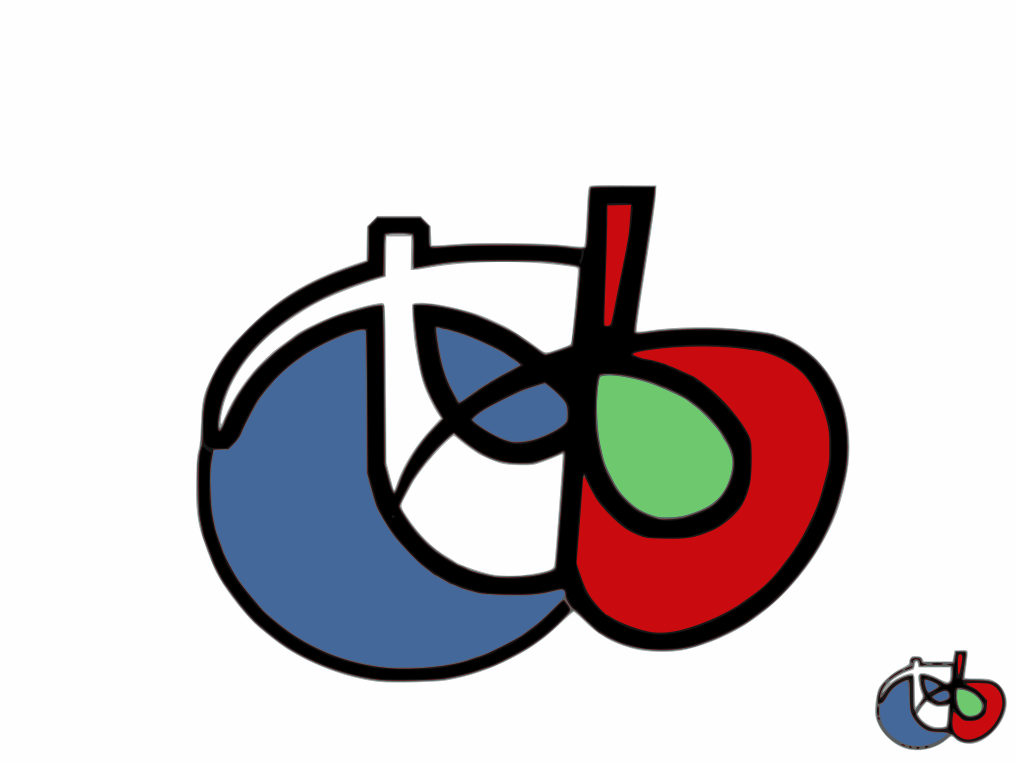
\includegraphics[width=0.5\textwidth]{../Art/logoVectoriel.pdf}
\large
\begin{center}
\emph{The ORFEO Toolbox is not a black box.}\\
\end{center}
\hspace{8cm} Ch.D.
\normalsize
\end{minipage}

%%%%%%%%%%%%%%%%%%%%%%%%%%%%%%%%%%%%%%%%%%%%%%
%
% remove headings from the following material
\pagestyle{plain}
%
%%%%%%%%%%%%%%%%%%%%%%%%%%%%%%%%%%%%%%%%%%%%%%

%%\ifitkPrintedVersion
%% \input{Cover.tex}
%%\fi

%\input{Abstract.tex}
\chapter*{Foreword}
\noindent

%%%%%%%%%%%%%%%%%%%%%%%%%%%%%%%%%%%%%%%%%%%%%%%%%%%%%%%%%
%
% Insert Table of Contents; List of Figures and Tables
%
%%%%%%%%%%%%%%%%%%%%%%%%%%%%%%%%%%%%%%%%%%%%%%%%%%%%%%%%%


%%%%%%%%%%%%%%%%%%%%%%%%%%%%%%%%%%%%%%%%%%%%%%
%
% enable headings from the following material
\pagestyle{normal}
%
%%%%%%%%%%%%%%%%%%%%%%%%%%%%%%%%%%%%%%%%%%%%%%
\small
\tableofcontents
\listoffigures
\listoftables
\normalsize

%%%%%%%%%%%%%%%%%%%%%%%%%%%%%%%%%%%%%%%%%
%
% Begin technical content
%
%%%%%%%%%%%%%%%%%%%%%%%%%%%%%%%%%%%%%%%%%

\mainmatter

\chapter{Introduction}

\chapter{Installation}

\chapter{OTB-Applications}

\chapter{Monteverdi}

\chapter{Recipes}

\section{Optical radiometric calibration}

\end{document}





\chapter{Applications Reference Documentation}\label{chap:apprefdoc}

This chapter is the reference applications documentation.

It provides detailed description of the application parameters, Python and bash snippets
to run the applications.

\input{ApplicationsReferenceAutoGen}


\end{document}



